\item \textbf{{[}NYJC/PRELIM/9569/2020/P2/Q3{]} }

You are to create a song playlist using a doubly linked list implemented
using Object-Oriented Programming (OOP). The doubly linked list data
structure is a linked list made up of nodes with two pointers pointing
to the next and previous element. 
\begin{center}
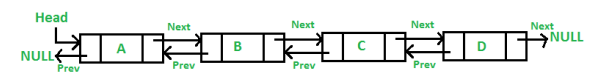
\includegraphics[width=0.5\paperwidth]{C:/Users/Admin/Desktop/Github/question_bank/LyX/static/img/9569-NYJC-2020-P2-Q3-1}
\par\end{center}

A doubly linked list allows traversal of nodes in both direction which
is not possible in a singly linked list. For example, a user can go
forward or backwards to play the next or previous song.

The \texttt{node}, will store the following data: 
\begin{itemize}
\item \texttt{title (str) }
\item \texttt{prev (node) }
\item \texttt{next (node)} 
\end{itemize}
The class, \texttt{SongPlaylist}, will store the following data: 
\begin{itemize}
\item a doubly linked list of \texttt{node} objects. 
\item \texttt{head} pointer, pointing to the first \texttt{node} in the
doubly linked list. 
\end{itemize}
The class \texttt{SongPlaylist} has the following methods: 
\begin{itemize}
\item \texttt{insert(SongPlaylist, title: str)} adds a song title at the
beginning of the list. 
\item \texttt{insertafter(SongPlaylist, searchtitle: str, newtitle: str)}
adds a song title after \texttt{searchtitle}.
\item \texttt{display(SongPlaylist)} outputs out the playlist. 
\end{itemize}
For each of the sub-tasks, add a comment statement, at the beginning
of the code using the hash symbol '\#', to indicate the sub-task the
program code belongs to, for example: 
\noindent \begin{center}
\begin{tabular}{c|l|}
\cline{2-2} 
\multirow{2}{*}{\texttt{In{[}1{]}:}} & \texttt{\# Task 3.1}\tabularnewline
 & \texttt{Program Code}\tabularnewline
\cline{2-2} 
\multirow{2}{*}{\texttt{In{[}2{]}:}} & \texttt{\# Task 3.2}\tabularnewline
 & \texttt{Program Code}\tabularnewline
\cline{2-2} 
\multirow{2}{*}{\texttt{In{[}3{]}:}} & \texttt{\# Task 3.3}\tabularnewline
 & \texttt{Program Code}\tabularnewline
\cline{2-2} 
\multicolumn{1}{c}{} & \multicolumn{1}{l}{\texttt{Output:}}\tabularnewline
\end{tabular}
\par\end{center}

\subsection*{Task 3.1 }

Write program code to define classes to implement the song playlist.
The figures below show the links that must be updated for the insert
and insertafter methods: 

Inserting at the beginning of the list
\begin{center}
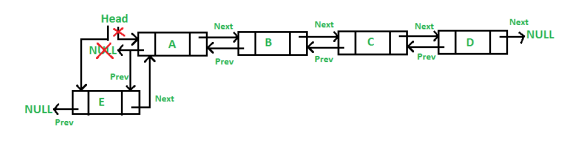
\includegraphics[width=0.5\paperwidth]{C:/Users/Admin/Desktop/Github/question_bank/LyX/static/img/9569-NYJC-2020-P2-Q3-2}
\par\end{center}

Inserting after a given node
\begin{center}
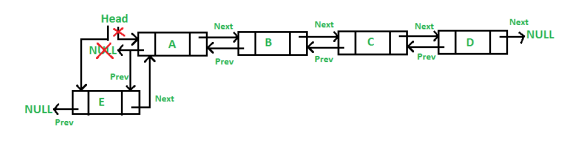
\includegraphics[width=0.5\paperwidth]{C:/Users/Admin/Desktop/Github/question_bank/LyX/static/img/9569-NYJC-2020-P2-Q3-3}
\par\end{center}

\noindent \begin{center}
\textcolor{white}{.}\hfill{}{[}10{]} 
\par\end{center}

The program has the following menu: 
\begin{enumerate}
\item[1.] \texttt{ Create New Song Playlist }
\item[2.] \texttt{ Add a song in front }
\item[3.] \texttt{ Add a song after }
\item[4.] \texttt{ Display Playlist }
\item[5.] \texttt{ -1 to End }
\end{enumerate}
Option 1 will prompt the user to enter the name of the new playlist. 

Option 2 will prompt the user to enter the song title and the name
of the playlist. 

Option 3 will prompt the user to enter the name of the playlist, existing
song title, and the new song title to be inserted after the existing
song title. 

Option 4 will prompt the user to enter the name of the playlist to
be displayed and output accordingly. 

\subsection*{Task 3.2 }

Write program code to: 
\begin{itemize}
\item display the main menu. 
\item input the choice by the user. 
\item run the appropriate code to carry out the task for the choice made.
\hfill{}{[}4{]}
\end{itemize}
Test your program by creating a new playlist called \texttt{MJ} and
add in the following titles in order: \texttt{\textquotedblleft Heal
the World\textquotedblright }, \texttt{\textquotedblleft Thriller\textquotedblright },
\texttt{\textquotedblleft Beat It\textquotedblright }. Show your output
by displaying the playlist.\hfill{}{[}2{]}

\subsection*{Task 3.3 }

Extend your program by writing a function \texttt{insertionSort(Playlist)}
that will sort the song titles in ascending order. 

The algorithm for this \texttt{insertionSort} is given below: 
\begin{enumerate}
\item[1)]  Create an empty \texttt{sorted} doubly linked list. 
\item[2)]  Traverse the given doubly linked list, do following for every node.
- Insert current node in sorted way in \texttt{sorted} doubly linked
list. 
\item[3)]  Change head of given linked list to head of \texttt{sorted} list. 
\end{enumerate}
Write program code to implement \texttt{insertionSort(Playlist)}.
\hfill{}{[}6{]}

Save your program code and output for Task 3 as 

\texttt{TASK3\_<your name>.ipynb}